
%%%%%%%%%%%%%%%%%%%%%%%%%%%%%%%%%%%%%%%%%%%%%%%%%%%%%%%%%%%%%%%%%%%%%%%%%%%%%%%%
\section{Introduction}
%%%%%%%%%%%%%%%%%%%%%%%%%%%%%%%%%%%%%%%%%%%%%%%%%%%%%%%%%%%%%%%%%%%%%%%%%%%%%%%%

Symbolic regression is an approach to interpretable machine learning in which the parameters, as well as the structure, of a model are optimized, typically with the goal of producing a model of a process that is easy to interpret, by virtue of its simplicity. 

Symbolic regression literature has, in general, fallen short of evaluating and/or identifying any method or family of methods that could conceivably be considered "state-of-the-art". 
In large part, these shortcomings are due to longstanding issues with the datasets used to benchmark symbolic regression, which are often small, trival, or simply not standardized (i.e. comparable) across papers or experiments~\cite{mcdermottGeneticProgrammingNeeds2012b}. 
Although community surveys~\cite{whiteBetterGPBenchmarks2012a,mcdermottGeneticProgrammingNeeds2012b} have led to suggestions for improving benchmarking standards, and even black-listed certain problems, contemporary literature continues to be published based on those datasets~\cite{petersenDeepSymbolicRegression2020}.
Furthermore, there is a stunning lack of cross-pollination between the research communities interested in symbolic regression, which include evolutionary computation, physics, engineering, statistics, and more traditional machine learning disciplines. 
Finally, lack of consensus on what SR methods constitute "state-of-the-art" is due in part to the ways in which methodological studies may be conducted - i.e., the relative merit of conducting incremental ablation studies versus large benchmark studies, such as this one. 
Whatever the causes, the result is that promising directions for future research in symbolic regression, and the outcomes that are possible, are not well supported by empirical evidence. 


The aspects of performance assessment for symbolic regression differ from typical regression benchmarking in important ways. 
For one, the competing objectives of accuracy and simplicity must be considered simultaneously.  
Furthermore, simplicity is itself a proxy for \textit{interpretability} - in other words, simplicity is often a necessary but not sufficient condition for interpretation.  
In this light, datasets with ground truth solutions are useful, in that they allow researchers to assess whether or not the symbolic model regressed by a given method is the exact solution. 
Assessing whether the symbolic model returned by a model is an exact match is non-trivial, and requires symbolic solvers with simplification procedures.
In addition, relative fidelity of estimated model forms that are not exact matches are difficult to assess.

Synthetic datasets with ground truth solutions are not sufficient for benchmarking symbolic regression algorithms. 
Such datasets do not give an adquate view into the expected performance of the algorithm when applied to datasets whose forms are yet to be discovered. 
Because of this, we consider it essential to also evaluate the performance of SR on real-world or otherwise black-box regression problems, relative to state-of-the-art ML methods. 

In this paper, we describe a large benchmarking effort that includes a dataset repository curated for symbolic regression, as well as a benchmarking repository designed to allow methodologists to easily contribute methods. 
We incorporated 130 new datasets with ground truth forms into the Penn Machine Learning Benchmark (PMLB)~\cite{olsonPMLBLargeBenchmark2017d}, including metadata describing the underlying equations, their units, and various summary statistics. 
Furthermore, we created a symbolic regression benchmark repository called SRBench\footnote{\url{https://github.com/EpistasisLab/srbench}} and sought contributions from researchers in this area. 
Here we describe this process and the results, which consist of comparisons of \hl{15} contemporary SR methods on hundreds of regression problems. 

To our knowledge this is by far the largest and most comprehensive SR benchmark effort to date, which allows us to make claims concering current state-of-the-art methods for SR with better certainty. 
Importantly, and in contrast to many previous efforts, the datasets, methods, benchmarking code, and results are completely open-source, reproducible, and revision-controlled, which should allow SRBench to exist as a living benchmark for future studies.

% New methods research risks falling into the trap of poor benchmarking strategies that have plagued previous symbolic regression efforts. 

%%%%%%%%%%%%%%%%%%%%%%%%%%%%%%%%%%%%%%%%%%%%%%%%%%%%%%%%%%%%%%%%%%%%%%%%%%%%%%%%
\section{Background and Motivation}
%%%%%%%%%%%%%%%%%%%%%%%%%%%%%%%%%%%%%%%%%%%%%%%%%%%%%%%%%%%%%%%%%%%%%%%%%%%%%%%%

\citet{kozaGeneticProgrammingProgramming1992a} introduced SR as an application of \textit{genetic programming} (GP), a field that investigates the use of genetic algorithms (GAs) to evolve executable data structures, i.e. programs. 
In the case of so-called ``Koza-style" GP, the programs to be optimized are syntax trees consisting of functions/operations over input features and constants. 
The earliest versions of GP used roulette-wheel selection to choose parents, and subtree mutation and subtree crossover to produce new variants (i.e. offspring) for the subsequent generation. 
Most SR research to date has emerged from within this subfield and its associated conferences (Genetic and Evolutionary Computation Conference (GECCO), )

Several recent works have proposed entirely different methods for tackling the SR problem. 
These include SR methods based in Bayesian optimization~\cite{jinBayesianSymbolicRegression2020}, recurrent neural networks (RNNs)~\cite{petersenDeepSymbolicRegression2020}, and physics-inspired divide-and-conquer strategies~\cite{udrescuAIFeynmanPhysicsInspired2020,udrescuAIFeynmanParetooptimal2020}. 

%% Eureqa, what it is and isn't
Some of these recent of these papers refer to Eureqa~\cite{schmidtDistillingFreeformNatural2009b}, a GP-based SR method used to re-discover known physics equations, as the "gold standard" for SR~\cite{petersenDeepSymbolicRegression2020} and/or the best method for SR "by far"~\cite{udrescuAIFeynmanPhysicsInspired2020}. 
On the basis of this claim, the aformentioned works present methods that out-perform Eureqa in terms of their ability to discover exact symbolic solutions to synthetic benchmark problems. 
However, \citet{schmidtDistillingFreeformNatural2009b} makes no claim to being the state-of-the-art method for SR, nor is this hypothesis tested in their study; in fact it is not the focus of any of the body of work on which it is based~\cite{schmidtMachineScienceAutomated2011}.  
Instead, Eureqa's development is rooted in a number of ablation studies, i.e. studies in which incremental algorithmic changes are presented and tested in controlled comparisons. 

The ``state-of-the-art" claim notwithstanding, Eureqa is certainly the most well-known and perhaps most commercially successful method for SR. 
Eureqa is a closed-source commercial software that was acquired by DataRobot in 2017\footnote{\url{https://www.datarobot.com/nutonian/}}. 
Due to its proprietary nature and incorporation into the DataRobot platform, it is impossible to benchmark its performance while controlling for important experimental variables such as computational effort. 
However, the algorithmic aspects of Eureqa are described in literature and summarized here. 
First is its use of directed acyclic graphs for representing equations in lieu of trees, which resulted in more space-efficient encodings without a significant difference in performance~\cite{schmidtComparisonTreeGraph2007}. 
The most significant improvement over traditional tournament-based selection is Eureqa's use of age-fitness Pareto optimization (AFP), a method in which random restarts are incorporated each generation as new offspring, and are protected from competing with older, more fit equations by including age as an objective to be minimized~\cite{schmidtAgefitnessParetoOptimization2011}. 
Eureqa also includes the co-evolution of fitness predictors, in which fitness assignment is sped up by optimizing a second population of training sample indices that best distinguish between equations in the population~\cite{schmidtCoevolutionFitnessPredictors2008}.
It is also possible that Eureqa no longer uses any of these reported algorithms for SR, due to its closed-source nature.
In that light, it is not clear what fundamental insight is gained when comparing to the software itself, other than a head-to-head comparison, since methodological insights cannot be extracted.

% New methods for symbolic regression
A close reading of SR literature since 2009 implies that a number of proposed methods would outperform Eureqa in controlled tests.
For one, AFP optimization has been outperformed by a number of semantic-aware selection methods (e.g.,~\cite{lacavaEpsilonLexicaseSelectionRegression2016c,liskowskiDiscoverySearchObjectives2017}), some of which are included in our study, alongside AFP.
Many other lines of research have pointed in promising directions, including hybridizations of GP with local search for constant optimization~\cite{topchyFasterGeneticProgramming2001,kommendaParameterIdentificationSymbolic2019} or structural tuning~\cite{lacavaInferenceCompactNonlinear2016}; the increasing use of semantic methods for guiding variation~\cite{moraglioGeometricSemanticGenetic2012a,virgolinLinearScalingSemantic2019} and selection~\cite{azadKrzysztofKrawiecBehavioral2017,lacavaProbabilisticMultiobjectiveAnalysis2019,arnaldoMultipleRegressionGenetic2014a}; and alternative representations of equations~\cite{defrancaInteractionTransformationEvolutionaryAlgorithm2020,mcconaghyFFXFastScalable2011}.

% lack of standards in symbolic regression field
The widespread adoption of these promising SR approaches is ham-strung by a lack of consensus on good benchmark problems, testing frameworks, and experimental designs. 
Our effort to establish a common benchmark is motivated by our view that the lack of strong, standardized benchmarks in the SR community impedes the adoption of promising techniques and impedes progress.  
As a counterexample, consider the comparatively quick adoption of advances in the neural network community that create a ratcheting effect of progress towards better methods and architectures. 
The quicker adoption of advancements for NNs is partially explained by the community's size, but we would contend that it is also due in part to community-wide focus on common benchmarks, frameworks (e.g. TensorFlow, PyTorch) and experiment designs. 
In comparison, in SR literature it is common to publish results on a small number of small, easy, and unrealistic problems, comparing only to very basic GP systems such as those described in~\cite{kozaGeneticProgrammingProgramming1992a} nearly thirty years ago.   
The issues around benchmarking have been described in detail~\cite{mcdermottGeneticProgrammingNeeds2012b}, and even led to community surveys and a proposal to ``black-list" several toy problems often reported in literature, such as the quartic polynomial problem~\cite{whiteBetterGPBenchmarks2012a}.
Despite these efforts to improve standards nearly ten years ago, toy datasets and comparisons to out-dated SR methods continue to appear in contemporary literature.

% efforts to benchmark SR
There have been recent efforts to improve benchmarking standards for SR.
\citet{zegklitzBenchmarkingStateoftheartSymbolic2020} benchmarked four SR methods (specifically those using linear regression) on five datasets. 
A larger benchmark (and precursor to this work) evaluated four recent SR methods on 94 regression problems in comparison to nine state-of-the-art ML approaches~\cite{orzechowskiWhereAreWe2018}. 
In both cases, SR methods were assessed solely on their ability to make accurate predictions. 
In contrast, \citet{udrescuAIFeynmanPhysicsInspired2020} proposed 120 new synthetic, physics-based datasets for SR, but compared only to Eureqa and only in terms of exact solutions. 
A major contribution of our work is its significantly more comprehensive scope than previous research.
We include \hl{15} SR methods on \hl{252} datasets in comparison to \hl{7} ML methods. 
Our comparisons are also more comprehensive: methods are benchmarked on their ability to generate models that are 1) accurate, 2) simple, and 3) exact or approximate symbolic matches to the ground truth process. 
In addition, we have made the benchmark openly available, reproducible, and open for contributions supported by continuous integration. 

% \subsection{Trends in Genetic Programming Literature}

% semantic methods

% parameter estimation 

% representation/encodings 

%%%%%%%%%%%%%%%%%%%%%%%%%%%%%%%%%%%%%%%%%%%%%%%%%%%%%%%%%%%%%%%%%%%%%%%%%%%%%%%%
\section{Methods}
%%%%%%%%%%%%%%%%%%%%%%%%%%%%%%%%%%%%%%%%%%%%%%%%%%%%%%%%%%%%%%%%%%%%%%%%%%%%%%%%

We created SRBench with the goal of having a living benchmarking of SR methods that invites rolling contributions. 
In order to establish common datasets, we extended PMLB, a standardized set of regression and classification problems\cite{olsonPMLBLargeBenchmark2017d}, by adding 130 SR datasets with known model forms. 
In order to standardize framework comparisons, we required contributors to define a minimal, Scikit-learn compatible~\cite{pedregosaScikitlearnMachineLearning2011a}, Python API for their method. 
An example contribution is shown in Figure~\ref{fig:ex_code}.

To ensure reproducibility, we defined a common environment (via conda) and with fixed versions of packages and their dependencies. 
We defined a continuous integration testing framework that tested the installation of new methods within this environment, and runs a set of tests to ensure new methods are compatible with the benchmark code.  
New contributions are submitted as pull requests and tested automatically.

We defined the experiment in two parts.
The first is a comparison of SR methods on ``black-box" regression problems, for which the metrics of interest are test set accuracy, model complexity, and training time. 
The second is a comparison of SR methods on ``ground-truth" regression problems, for which the metrics of interest are exact solution rates, test set accuracy, model complexity, and training time. 


\paragraph{Accuracy}
We assessed accuracy using the coefficient of determination ($R^2$), defined as 

\begin{equation}
    R^2 = 1 - \frac{\sum_i^N{(y_i - \hat{y}_i)^2}}
                   {\sum_i^N{(y_i - \bar{y}_i)^2}}
\end{equation}

%%
% complexity
%%
\paragraph{Complexity}
A number of different complexity measures have been proposed for SR, including those based in \textit{syntactic} complexity (i.e. related to the complexity of the symbolic model), \textit{semantic} complexity (i.e. related to the behavior of the model over the data)~\cite{vladislavlevaOrderNonlinearityComplexity2009a,udrescuAIFeynmanParetooptimal2020}, or both~\cite{kommendamichaelEvolvingSimpleSymbolic2015}. 
The pros and cons of these methods and their relation to generalization and interpretability is discussed frequently in literature~\cite{murdochDefinitionsMethodsApplications2019}. 
For the sake of simplicity, we opted to define complexity as the number of simple mathematical operators, nodes and constants in the model, where simple mathematical operators are in the set 
$\{+,
    -,
    *,
    {/},
    \sin,
    \cos,
    \arcsin,
    \arccos,
    \exp,
    \log, 
\text{pow},
\max,
\min \}$. 
In addition to calculating the complexity of the raw model forms returned by each method, we calculated the complexity of the models after simplifying via \href{https://www.sympy.org/en/index.html}{sympy}.

%%
% solutions
%%%
\paragraph{Solution Criteria}
For the ground truth regression problems, we evaluated whether the final model was a ``solution" to the task according to two metrics: \textit{accuracy solution} and \textit{symbolic solution}. 
A final model was considered an accuracy solution if it had a (near) perfect accuracy on the test set, defined as $R^2>0.999$. 
A model was considered a symbolic solution if it was non-constant and satisifed at least one of the following conditions: 

\begin{enumerate}
    \item $\phi^*-\hat{\phi} = c $
    \item $\frac{\phi^*}{\hat{\phi}} = c $ 
\end{enumerate}

where $c$ is a constant. 
This definition is designed to capture models within an affine transformation of the true model form (those that differ only by a constant or scalar). 
Prior to assessing symbolic solutions, each model underwent sympy simplification, as did the conditions above. 
We chose to report both of these solution definitions because there are pros and cons to both. 
Symbolic solutions are preferable to accuracy solutions in the sense that they are more a more faithful evaluation of the ability of an SR method to discover the data generating process.
However, because any symbolic function can be represented in an infinite number of ways, and sympy's simplification procedure uses non-optimal heuristics, we cannot guarantee that all symbolic solutions are captured with perfect fidelity by this metric. 
The accuracy solution metric more explicitly measures the model's ability to perfectly capture the underlying process, yet it has the disadvantage of being reported over finite samples. 
Therefore accuracy solutions may not truly capture the data generating process. 
In this sense, one may view the accuracy solution and symbolic solution metrics as optimistic and pessimistic estimates of performance, respectively.

\subsection{SR Methods}

We evaluated a number of SR algorithms in this benchmark that are summarized in Table~\ref{tbl:methods}.
Here we briefly describe what these methods are and describe how they fit into broader research trends within the SR field. 

% table of methods
\begin{table}
    \footnotesize
    \center
    \caption{
        Short descriptions of the SR methods benchmarked in our experiment, including references and links to implementations. 
    }\label{tbl:methods}
    \rowcolors{2}{gray!25}{white}
    \begin{tabular}{l L{12em} L{8em} r}
        \rowcolor{white}
        Method      &   Description                                         &   Method Family                       &   Implementation  \\ 
        \midrule
        AFP~\cite{schmidtAgefitnessParetoOptimization2011}               &   Age-fitness Pareto Optimization     &   GP
                    &   C++/Python (\href{https://github.com/EpistasisLab/ellyn}{link})                  \\
        AIFeynman~\cite{udrescuAIFeynmanParetooptimal2020}               &   Physics-inspired method             &   Divide and conquer
                    &   Fortran/Python (\href{https://github.com/SJ001/AI-Feynman}{link})              \\
        BSR~\cite{jinBayesianSymbolicRegression2020}                     &   Bayesian Symbolic Regression        &   Markov Chain Monte Carlo
                    &   Python (\href{https://github.com/ying531/MCMC-SymReg}{link})                      \\
        DSR~\cite{petersenDeepSymbolicRegression2020}                    &   Deep Symbolic Regression            &   Recurrent neural networks   
                    &   Python (PyTorch) (\href{https://github.com/brendenpetersen/deep-symbolic-regression}{link})            \\
        EPLEX~\cite{lacavaProbabilisticMultiobjectiveAnalysis2019}       &   $\epsilon$-lexicase selection       &   GP
                    &   C++/Python (\href{https://github.com/EpistasisLab/ellyn}{link})                  \\
        FEAT~\cite{lacavaLearningConciseRepresentations2019c}        &   Feature Engineering Automation Tool &   GP                          
                    &   C++/Python (\href{https://github.com/lacava/feat}{link})                  \\
        AFP\_FE~\cite{schmidtDistillingFreeformNatural2009b}               &   AFP with co-evolved fitness estimates; Eureqa-esque     &   GP
                    &   C++/Python (\href{https://github.com/EpistasisLab/ellyn}{link})                  \\
        FFX~\cite{mcconaghyFFXFastScalable2011}         &   Fast function extraction             &   Random search               
                    &   C++/Python (\href{https://github.com/natekupp/ffx/tree/master/ffx}{link})                  \\
        GPGOMEA~\cite{virgolin2020improving}     &   Gene-pool Optimal Mixing Evolutionary Algorithm     & GP            
                    &   C++/Python (\href{https://github.com/marcovirgolin/GP-GOMEA/}{link})                  \\
        gplearn     &   Koza-style symbolic regression in Python       &   GP                          
                    &   C++/Python (\href{https://github.com/trevorstephens/gplearn}{link})                  \\
        ITEA~\cite{defrancaInteractionTransformationEvolutionaryAlgorithm2020}   &   Interaction-Transformation EA       &   GP
                    &   Haskell/Python (\href{https://github.com/folivetti/ITEA/}{link})              \\
        MRGP~\cite{arnaldoMultipleRegressionGenetic2014a}                        &   Multiple Regression Genetic Programming &   GP
                    &   Java (\href{https://github.com/flexgp/gp-learners}{link})                        \\
        Operon~\cite{kommendaParameterIdentificationSymbolic2019}                &   SR with Non-linear least squares     &   GP
                    &   C++/Python (\href{https://github.com/heal-research/operon}{link})                  \\
        SemBackProp~\cite{virgolinLinearScalingSemantic2019}                     &   Semantic Back-propagation           &   GP
                    &   C++/Python (\href{https://github.com/marcovirgolin/GP-GOMEA}{link})                  \\ 
        \bottomrule
    \end{tabular}
\end{table}



\subsubsection{Genetic Programming-Based Methods}

Most methods for SR come from the genetic programming (GP) literature. 
The canonical implementation of GP-based SR starts with an initially random population programs/models, and then iterates through the steps of selection, variation and (optionally) survival~\cite{poliFieldGuideGenetic2008}.
Selection chooses individuals from which to produce new points in the search space in the subsequent iteration. 
The de-facto method of selection is tournament selection, in which a fixed-size sample of individuals are drawn and the fittest individual chosen as winner. 
Selected models then under-go some combination of randomized mutation and/or crossover, traditionally at the subtree level or single node level.
In Koza-style GP, the resulting offspring replace the parents, but several common methods include a survival step in which the resulting offspring compete against the parents, at the very least to ensure the best model in the search space is not lost.

Given these basic components, we can categorize contemporary methods based on the steps which they target - i.e. selection, variation, survival, or fitness/evalaution. 


\paragraph{Epsilon-lexicase selection}

One selection that has emerged as an improvement over tournament selection and AFP is $\epsilon$-lexicase selection (EPLEX)~\cite{lacavaEpsilonLexicaseSelectionRegression2016c}. 
Rather than aggregating the training loss across samples, EPLEX utilizes the error vectors to conduct selection as if through a series of filters. 
We benchmark EPLEX as a stand-alone change, but it also appears as the parent selection method in FEAT~\cite{lacavaLearningConciseRepresentations2019c}. 

\paragraph{Semantic Backpropagation}

Semantic backpropagation (SB) is a technique invented and popularized by~\cite{wieloch2013running,krawiec2013approximating,pawlak2014semantic} to compute, for a given target value and a tree node position, what output is needed at the given position to make the output of the tree match the target value (see Fig. 1). 
It works by iterative inversions of the ancestry of function nodes, from the root down to the chosen node position. 
Here, we rely on the algorithm by~\citet{virgolinLinearScalingSemantic2019}, an SB -based GP which is capable to tackle real-world regression datasets. 
In this algorithm, similarly to~\cite{wieloch2013running}, recombination improves a solution by applying SB on a random node position and using the label as target, and replacing the subtree rooted at the sampled position with a tree chosen from a pre-computed library. 
The chosen tree has output that best matches the one computed by SB (i.e., using the Euclidean distance on output vectors defined over the training set). 
Moreover, optimal affine transformations are computed at the start of SB and during library parsing, resulting in substantial performance gains~\cite{virgolinLinearScalingSemantic2019}.

\paragraph{Constant optimization}
Traditional GP encodes constants as building blocks that are initialized from a given distribution, and then optimizes them through the same process as the rest of the component building blocks.
One of the clearest improvements over Koza-style GP has been the adoption of local search methods to handle constant optimization distinctly from evolutionary learning. 
Backpropagation-based gradient descent has been proposed for GP-SR by~\citet{topchyFasterGeneticProgramming2001}, but for years was not widely adopted. 
For example, the methods of~\citet{bongardNonlinearSystemIdentification2005a} and~\citet{schmidtDistillingFreeformNatural2009} that would appear years later opted for stochastic hill climbing for handling constant optimization. 
More recent studies by~\cite{kommenda_effects_2013,kommendaParameterIdentificationSymbolic2019} have made a strong case for the use of non-linear least squares approaches to constant optimization, and establish gradient-based constant optimization as an improvement over random or evoluationary approaches.

In addition to the question of how to best optimize constants, a line of research has proposed improved ways of defining constants within or between program encodings. 
Rather than treating constants as building blocks, FEAT~\cite{lacavaLearningConciseRepresentations2019c} and Operon~\cite{burlacuOperonEfficientGenetic2020} encode weights at the edges of all nodes. 
MRGP~\cite{arnaldoMultipleRegressionGenetic2014a} splays individual program stack trace out as a matrix, using Lasso to identify building blocks and to train the final model.
Methods such as FFX~\cite{mcconaghyFFXFastScalable2011}, EFS~\cite{arnaldoBuildingPredictiveModels2015}, and FEW~\cite{lacavaGeneralFeatureEngineering2017} treat the entire population as a single model for which individuals are features.

\paragraph{Gene-pool Optimal Mixing Evolutionary Algorithm}

The Genetic Programming version of the Gene-pool Optimal Mixing Evolutionary Algorithm (GP-GOMEA) is an EA with adaptive recombination based on a \emph{linkage model}~\cite{virgolin2017scalable,virgolin2020improving}. 
A linkage model is a model of the level of interdependencies (i.e., linkage) existing within the encoding of evolving solutions~\cite{thierens2011optimal}. 
Like other algorithms of the GOMEA family, GP-GOMEA computes a linkage model every generation, and uses this information to guide its recombination phase. 
The goal is to prevent the disruption potentially-salient patterns of components, i.e., \emph{building blocks} with a positive concerted action.
In~\cite{virgolin2017scalable,virgolin2020improving}, it was shown that GP-GOMEA’s linkage-based recombination works significantly better than random recombination, and is especially competitive when small, potentially interpretable solutions are sought. 
We use the same implementation of~\cite{virgolin2020improving}.

\paragraph{Bayesian Symbolic Regression}

\citet{jinBayesianSymbolicRegression2020} recently proposed Bayesian Symbolic Regression (BSR), in which a prior is placed on tree structures and the posterior distributions are sampled using a Markov Chain Monte Carlo (MCMC) method.   
As in GP-based SR, arithmetic expressions are expressed with symbolic trees, although BSR explicitly defines the final model form as a linear combination of several symbolic trees. 
Model parsimony is encouraged by specifying a prior that presumes additive, linear combinations of small components. 

\paragraph{Deep Symbolic Regression}
Deep Symbolic Regression (DSR)~\cite{petersenDeepSymbolicRegression2020} 
DSR showed good performance in finding exact solutions to a number of synthetic benchmark problems, although 6 of the 12 problems for which they reported results in the main text (c.f. Table 1,~\cite{petersenDeepSymbolicRegression2020}) are low-order synthetic polynomials that were proposed for black-listing in~\citet{whiteBetterGPBenchmarks2012a} (c.f. Table 3).  


\paragraph{AI-Feynman}

%%%%%%%%%%%%%%%%%%%%%%%%%%%%%%%%%%%%%%%%%%%%%%%%%%%%%%%%%%%%%%%%%%%%%%%%%%%%%%%%
\section{Experimental Setup}
%%%%%%%%%%%%%%%%%%%%%%%%%%%%%%%%%%%%%%%%%%%%%%%%%%%%%%%%%%%%%%%%%%%%%%%%%%%%%%%%

We evaluated SR methods on two separate tasks. 
First, we assessed their ability to make accurate predictions on "black-box" regression problems while minimizing the syntactic complexity of the solution. 
Here "black-box" refers to not knowing the functional form of the underlying data-generating process, assuming one exists.   
Second, we tested the ability of each method to find exact solutions to synthetic datasets with known, ground-truth functions. 
The second set of problems are based on physics equations from several sources, as described below. 

The basic experiment settings are summarized in Table~\ref{tbl:exp}.

\begin{table}
    \footnotesize
    \center
    \caption{
        Settings used in the benchmark experiments. 
        ``Total comparisons" refers to the total evaluatons of an algorithm on a dataset for a given noise level and random seed.
    }\label{tbl:exp}
    % \rowcolors{2}{gray!25}{white}
    \begin{tabular}{lll}
        Setting                     &   Black-box Problems              &   Ground-truth Problems                   \\
        \midrule
        No. of datasets             &   122                             &   130                                     \\
        No. of algorithms           &   21 (14 SR, 7 ML)                &   14                                      \\
        No. of trials per dataset   &   10                              &   10                                      \\
        Train/test Split            &   .75/.25                         &   .75/.25                                 \\
        Hyperparameter Tuning       &   5-fold Halving Grid Search CV   &   None (best set from BB problems)        \\
        Termination criteria        &   500k evaluations/train or 48 hours    &   1M evaluations or 8 hours         \\ 
        Levels of target noise      &   None                            &   0, 0.001, 0.01                          \\
        Total comparisons           &   26840                           &   54600                                   \\ 
        \bottomrule
    \end{tabular}
\end{table}


\subsection{Black-box Regression Problems}

We used \hl{122} black-box regression problems available in PMLB v.1.0. 
These problems are pulled from, and overlap with, varous open-source repositories, including OpenML~\cite{vanschorenOpenMLNetworkedScience2013} and the UCI repository~\cite{lichmanUCIMachineLearning2013a}. 
PMLB standardizes these datasets to a common format and provides fetching functions to load them into Python (and R). 
Each dataset includes metadata describing source information as well as a profile detailing the data distributions (e.g. \href{https://epistasislab.github.io/pmlb/profile/analcatdata_aids.html}{this dataset}).


\subsection{Ground-Truth Regression Problems}
We extended PMLB with 130 datasets with known, ground-truth model forms. 
These datasets were used to assess the ability of SR methods to recover known process physics. 
The 130 datasets came from two sources: the \href{https://space.mit.edu/home/tegmark/aifeynman.html}{Feynman Symbolic Regression Database}, 
and the \href{https://github.com/lacava/ode-strogatz}{ODE-Strogatz repository}.

Both sets of data come from first principles models of physical systems. 
The Feynman datasets created and studied by~\citet{udrescuAIFeynmanPhysicsInspired2020}, and the Strogatz datasets 
Each dataset is one state of a 2-state system of first-order, ordinary differential equations (ODEs). 

extend \hl{122} black-box regression problems available in PMLB v.1.0. 
These problems are pulled from, and overlap with, varous open-source repositories, including OpenML~\cite{vanschorenOpenMLNetworkedScience2013} and the UCI repository~\cite{lichmanUCIMachineLearning2013a}. 
PMLB standardizes these datasets to a common format and provides fetching functions to load them into Python (and R). 
Each dataset includes metadata describing source information as well as a profile detailing the data distributions (e.g. \href{https://epistasislab.github.io/pmlb/profile/analcatdata_aids.html}{this dataset}).

%%%%%%%%%%%%%%%%%%%%%%%%%%%%%%%%%%%%%%%%%%%%%%%%%%%%%%%%%%%%%%%%%%%%%%%%%%%%%%%%
\section{Results}
%%%%%%%%%%%%%%%%%%%%%%%%%%%%%%%%%%%%%%%%%%%%%%%%%%%%%%%%%%%%%%%%%%%%%%%%%%%%%%%%

\subsection{Black-box Regression Problems}
% overall pmlb results
\begin{figure}
    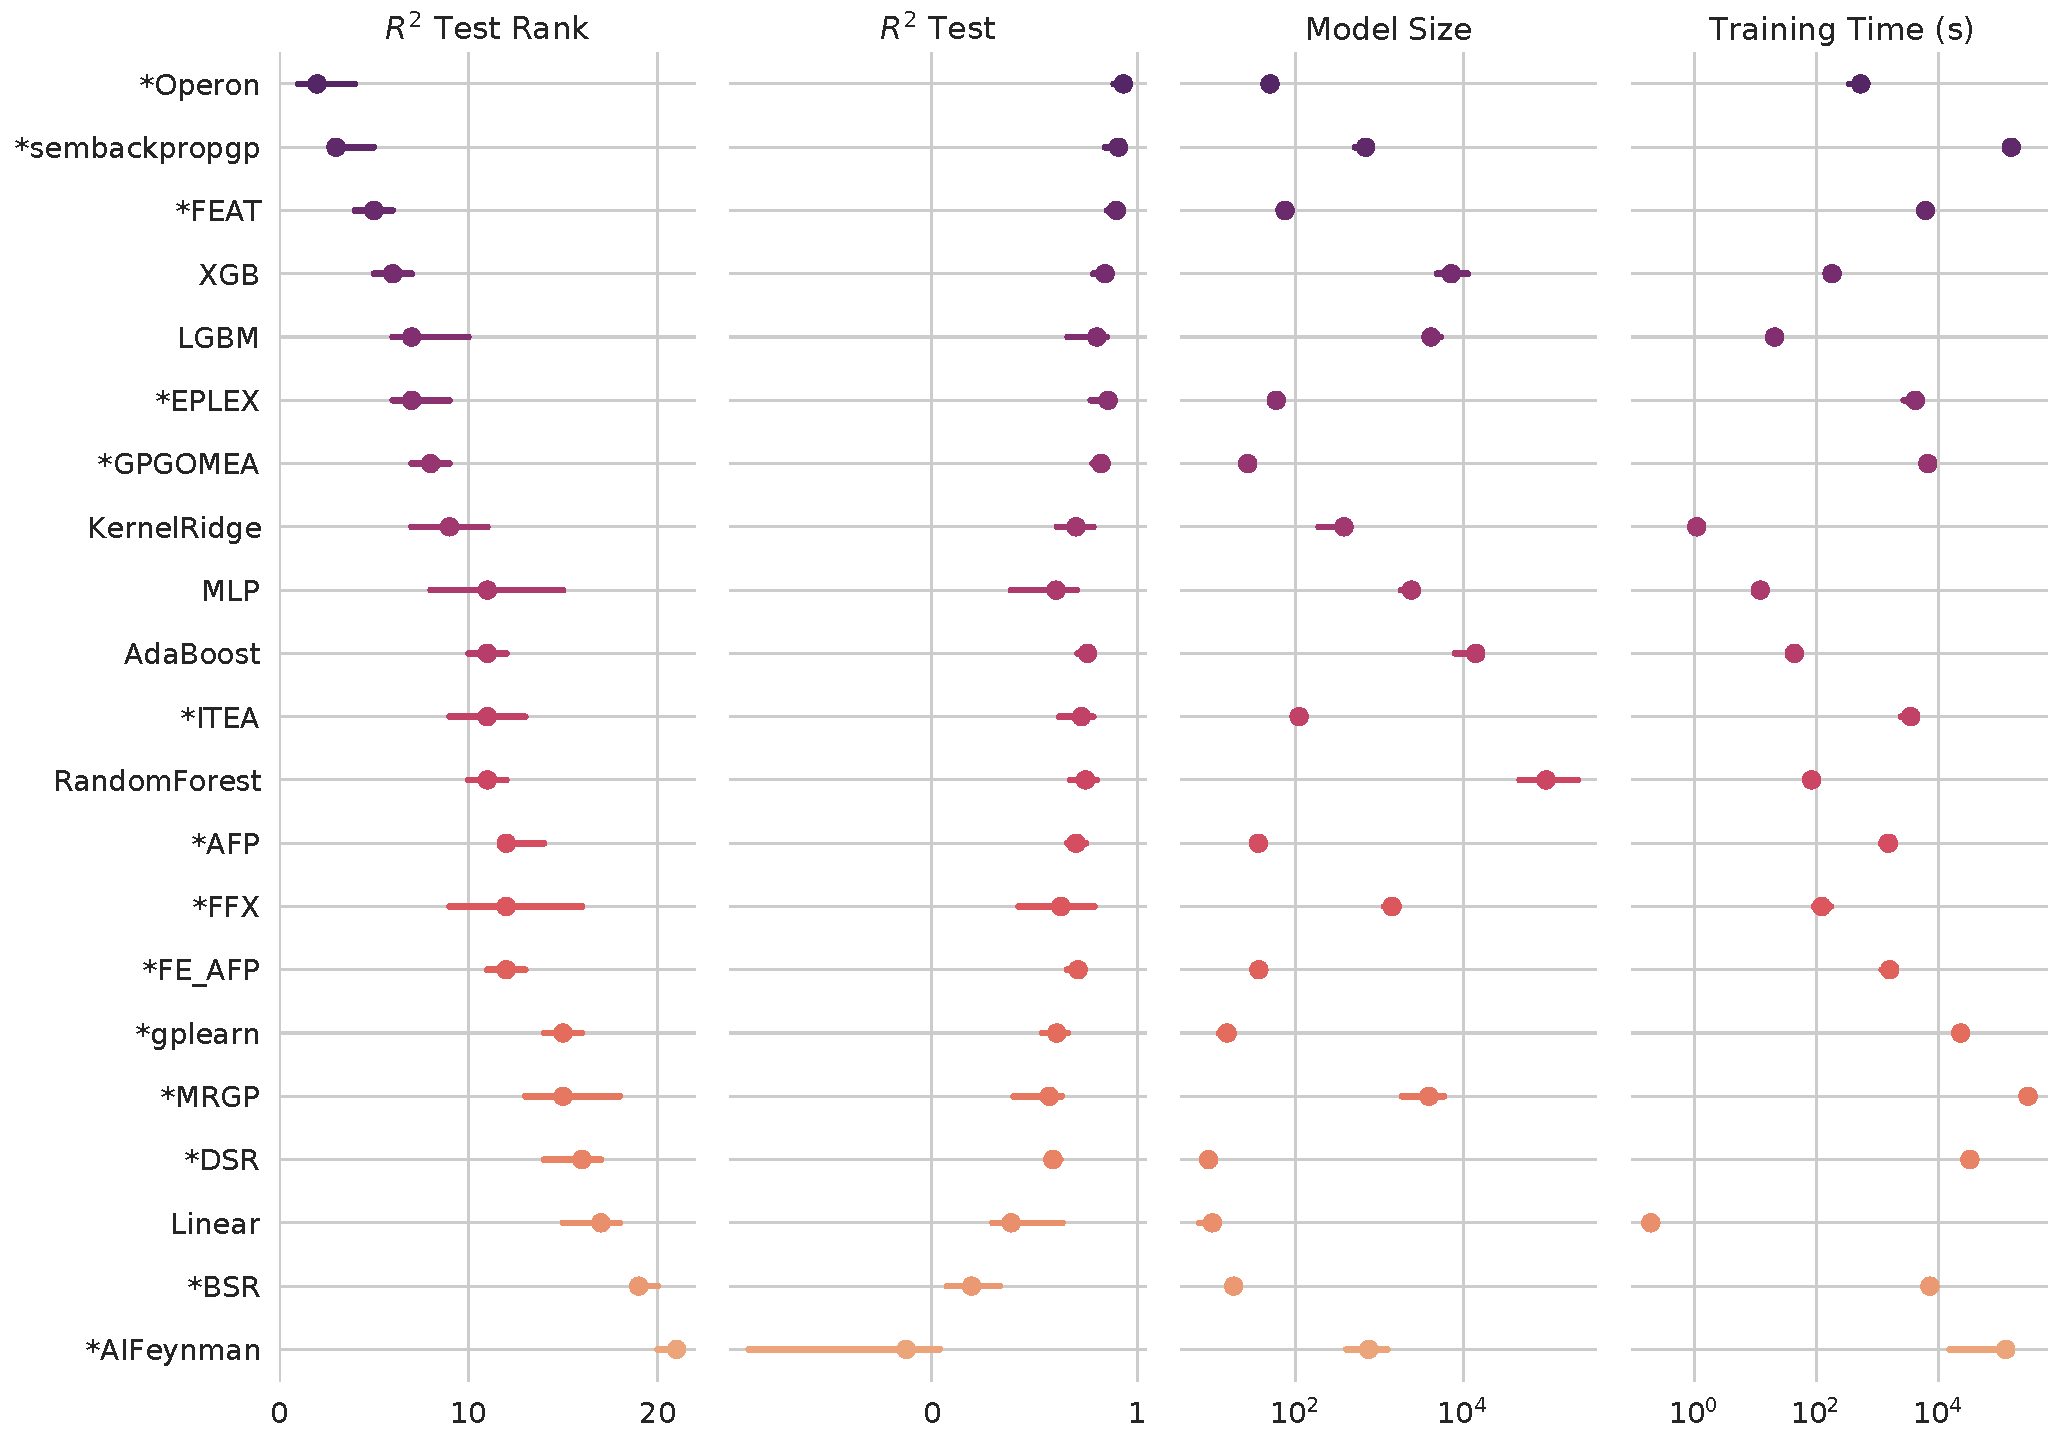
\includegraphics[width=\textwidth]{figs/results_pmlb_r1/pairgrid-pointplot_r2_test_rank_r2_test_model_size_training-time-(s).pdf}
    \caption{ 
        Results on the black-box regression problems.
        Points indicate the mean of the median test set performance on all problems, and bars show the 95\% confidence interval. 
        Methods marked with an asertisk are SR methods. 
    }
    \label{fig:pmlb_perf}
\end{figure}

\subsection{Ground-Truth Regression Problems}
% solutions in terms of perfect accuracy, perfect models
% success rates

\begin{figure}
    \centering
    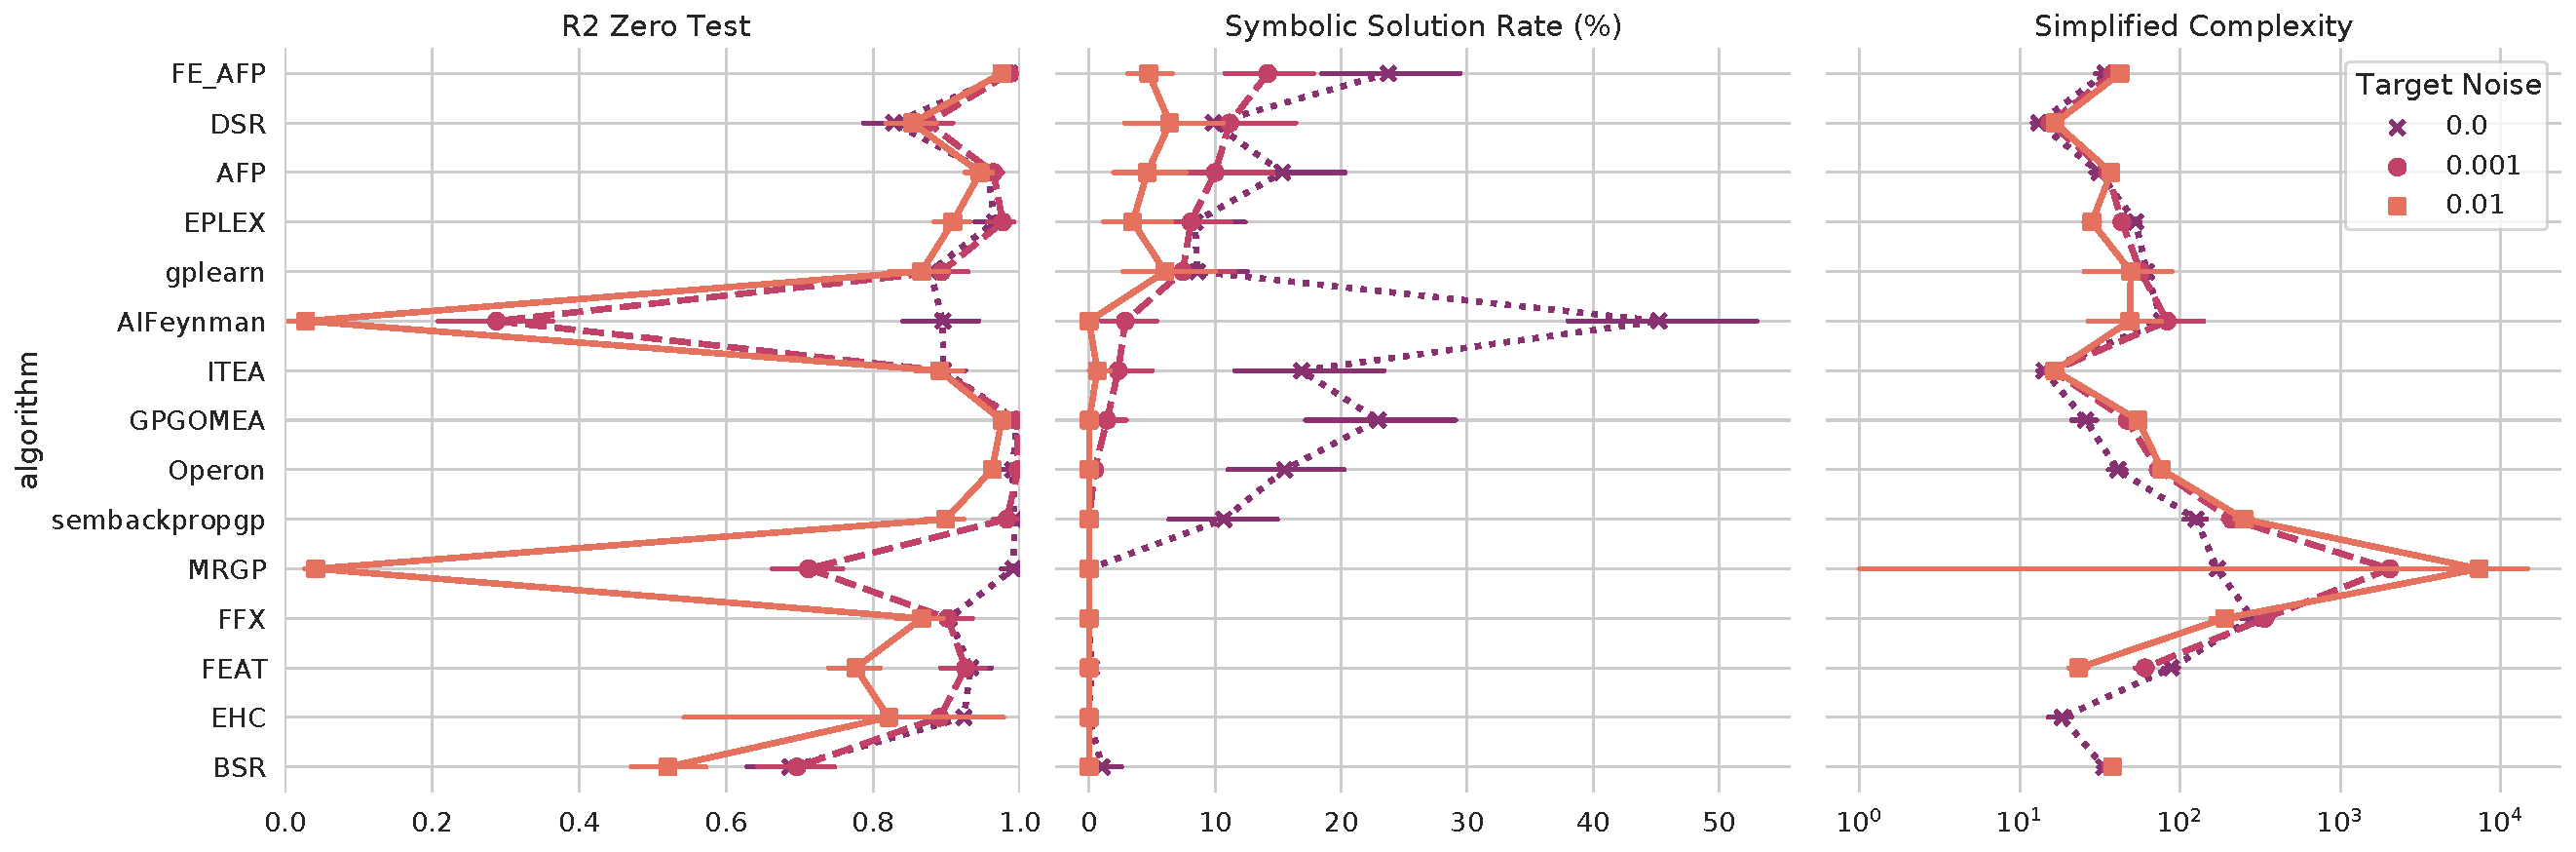
\includegraphics[width=\textwidth]{figs/results_sym_data/pairgrid_r2_zero_test_symbolic_solution_rate_(pct)_simplified_complexity.pdf}
    % \begin{minipage}{0.49\textwidth}
    %     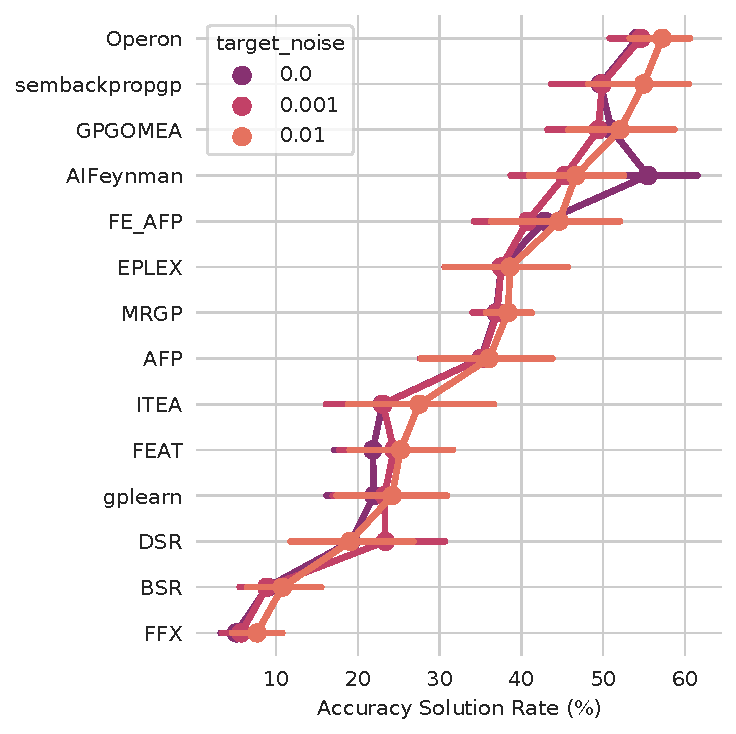
\includegraphics[width=\textwidth]{figs/results_sym_data/cat-pointplot-Accuracy-Solution-Rate-(pct)-by-Algorithm.pdf}
    % \end{minipage}
    % % \hspace{0.01\textwidth}
    % \begin{minipage}{0.49\textwidth}
    %     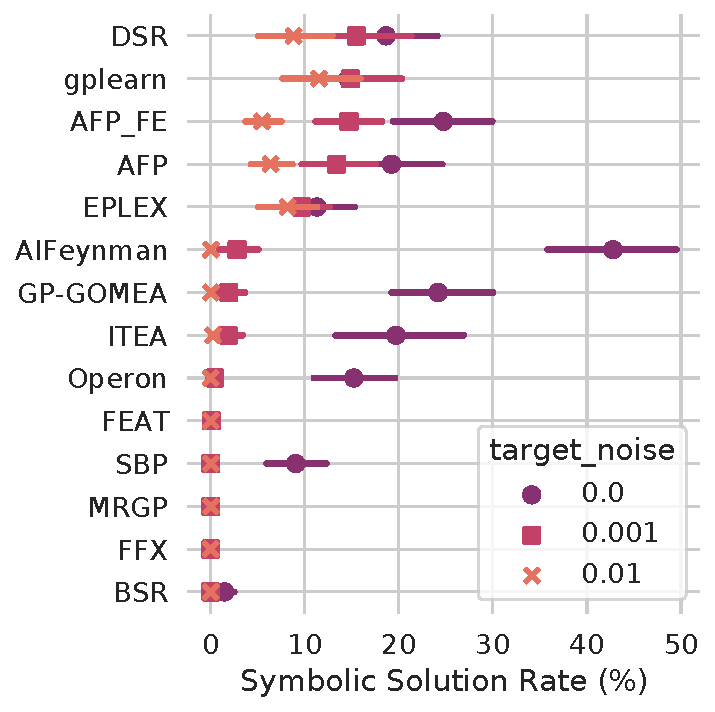
\includegraphics[width=\textwidth]{figs/results_sym_data/cat-pointplot-Symbolic-Solution-Rate-(pct)-by-Algorithm.pdf}
    % \end{minipage}
    \caption{
        Solution rates in terms of perfect accuracy (Left) versus symbolic equivalence (Right) for the Feynman and Strogatz problems. 
        Color indicates level of noise added to the target variable. 
    }
    \label{fig:symbolic_solns}
\end{figure}

% runtime, complexity 
% pareto curves
Since we are concerned with accuracy as well as simplicity, we take "state-of-the-art" to mean methods that are on the Pareto front of accuracy and simplicity. 
We estimate and visualize the Pareto front for black-box and ground-truth regression in Figure~\ref{fig:pareto}. 

\begin{wrapfigure}{r}{0.6\textwidth}
    \centering
    % \begin{minipage}{0.49\textwidth}
    \includegraphics[width=0.5\textwidth]{figs/results_pmlb_r1/pareto_plot_r2_test_rank_model_size_rank.pdf}
    % \end{minipage}
    % \hspace{0.01\textwidth}
    % \begin{minipage}{0.49\textwidth}
    %     \includegraphics[width=\textwidth]{figs/results_sym_data/pareto_plot_r2_test_rank_model_size_rank.pdf}
    % \end{minipage}
    \caption{
        Pareto plots comparing the rankings of SR methods in terms of model size and $R^2$ score; (left) black-box problems, (right) ground-truth problems.
        Points are the median ranking across datasets, and the bars represent 95\% confidence intervals. 
    } \label{fig:pareto}
\end{wrapfigure}

%%%%%%%%%%%%%%%%%%%%%%%%%%%%%%%%%%%%%%%%%%%%%%%%%%%%%%%%%%%%%%%%%%%%%%%%%%%%%%%%
\section{Discussion and Conclusions}
%%%%%%%%%%%%%%%%%%%%%%%%%%%%%%%%%%%%%%%%%%%%%%%%%%%%%%%%%%%%%%%%%%%%%%%%%%%%%%%%

\subsection{Directions for improvement in SR}

\paragraph{Tolerance to noise}
